\documentclass[pdflatex,sn-mathphys]{sn-jnl}
\jyear{\year}

\usepackage{lipsum}

\raggedbottom

\begin{document}

\title[Modelagem de planta industrial]{Modelagem de planta industrial}

%%=============================================================%%
%% Prefix	-> \pfx{Dr}
%% GivenName	-> \fnm{Joergen W.}
%% Particle	-> \spfx{van der} -> surname prefix
%% FamilyName	-> \sur{Ploeg}
%% Suffix	-> \sfx{IV}
%% NatureName	-> \tanm{Poet Laureate} -> Title after name
%% Degrees	-> \dgr{MSc, PhD}
%% \author*[1,2]{\pfx{Dr} \fnm{Joergen W.} \spfx{van der} \sur{Ploeg} \sfx{IV} \tanm{Poet Laureate} 
%%                 \dgr{MSc, PhD}}\email{iauthor@gmail.com}
%%=============================================================%%

\author*[1]{\fnm{First} \sur{Author}}\email{First@gmail.com}

\author[2,3]{\fnm{Second} \sur{Author}}\email{iiauthor@gmail.com}
\equalcont{These authors contributed equally to this work.}

\author[1,2]{\fnm{Third} \sur{Author}}\email{iiiauthor@gmail.com}
\equalcont{These authors contributed equally to this work.}

\affil*[1]{\orgdiv{PPGEE}, \orgname{UTFPR}, \orgaddress{\street{Via do Conhecimento}, \city{Pato Branco}, \postcode{85503-390}, \state{PR}, \country{Brasil}}}

\affil[2]{\orgdiv{Department}, \orgname{Organization}, \orgaddress{\street{Street}, \city{City}, \postcode{10587}, \state{State}, \country{Country}}}

\affil[3]{\orgdiv{Department}, \orgname{Organization}, \orgaddress{\street{Street}, \city{City}, \postcode{610101}, \state{State}, \country{Country}}}



\abstract{The abstract serves both as a general introduction to the topic and as a brief, non-technical summary of the main results and their implications. Authors are advised to check the author instructions for the journal they are submitting to for word limits and if structural elements like subheadings, citations, or equations are permitted.}

\keywords{keyword1, Keyword2, Keyword3, Keyword4}

%%\pacs[JEL Classification]{D8, H51}

%%\pacs[MSC Classification]{35A01, 65L10, 65L12, 65L20, 65L70}

\maketitle

\section{Plantas}
Robo 1
\lipsum[1]
\begin{figure}[H]%
    \centering
    \includegraphics[width=0.9\textwidth]{imagens/robo_1.eps}
    \caption{Planta Robo 1}\label{fig:robo1}
\end{figure}

Robo 2
\lipsum[2]
\begin{figure}[H]%
    \centering
    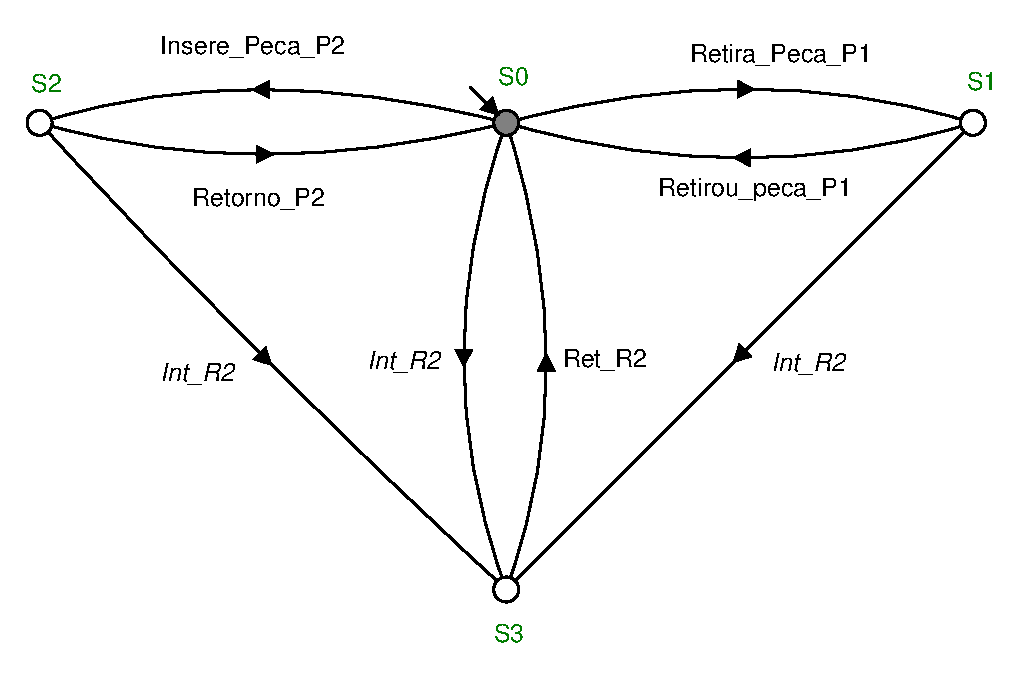
\includegraphics[width=0.9\textwidth]{imagens/robo_2.eps}
    \caption{Planta Robo 2}\label{fig:robo2}
\end{figure}

Robo 3
\lipsum[3]
\begin{figure}[H]%
    \centering
    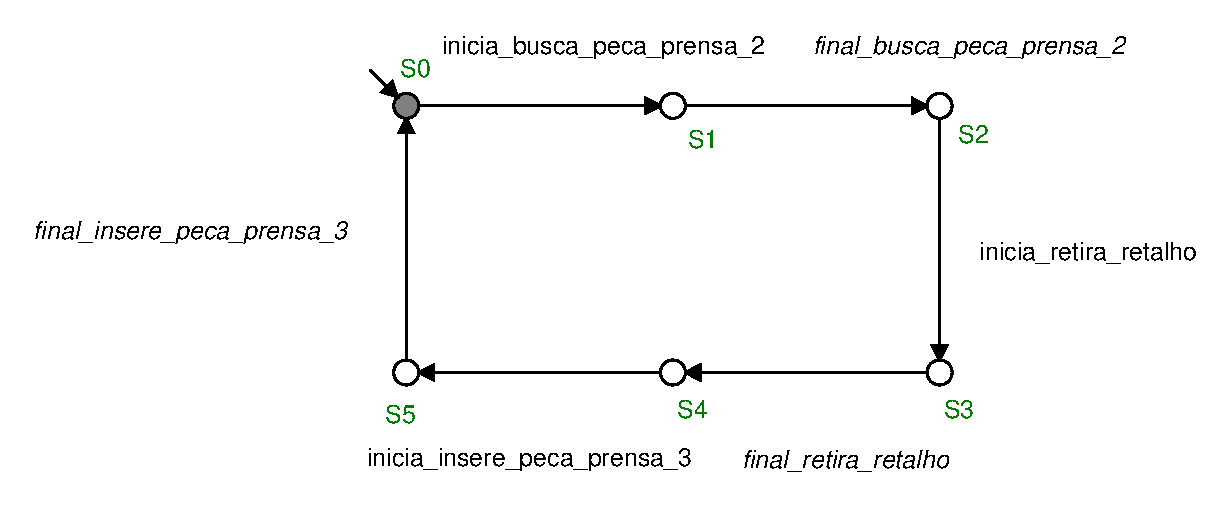
\includegraphics[width=0.9\textwidth]{imagens/robo_3.eps}
    \caption{Planta Robo 3}\label{fig:robo3}
\end{figure}

Robo 4
\lipsum[4]
\begin{figure}[H]%
    \centering
    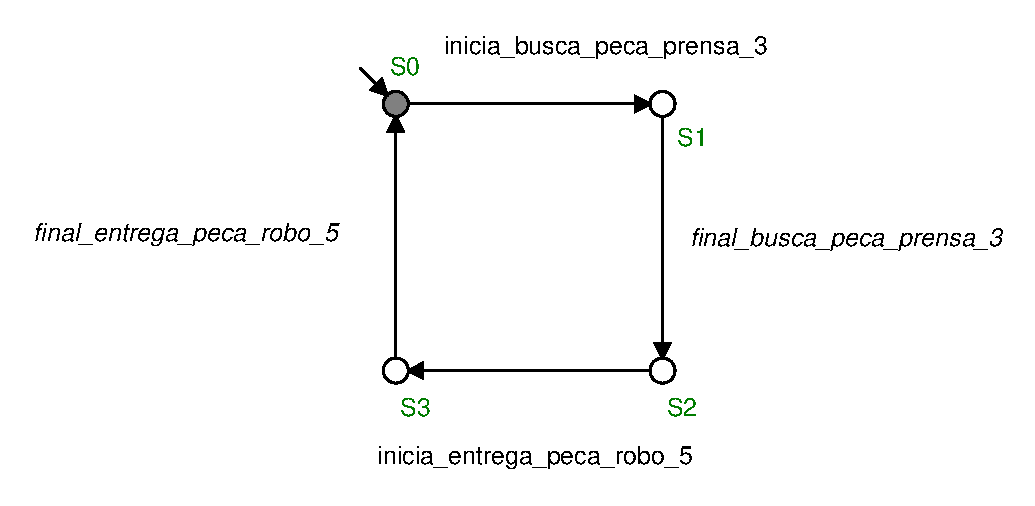
\includegraphics[width=0.9\textwidth]{imagens/robo_4.eps}
    \caption{Planta Robo 4}\label{fig:robo4}
\end{figure}

Robo 5
\lipsum[5]
\begin{figure}[H]%
    \centering
    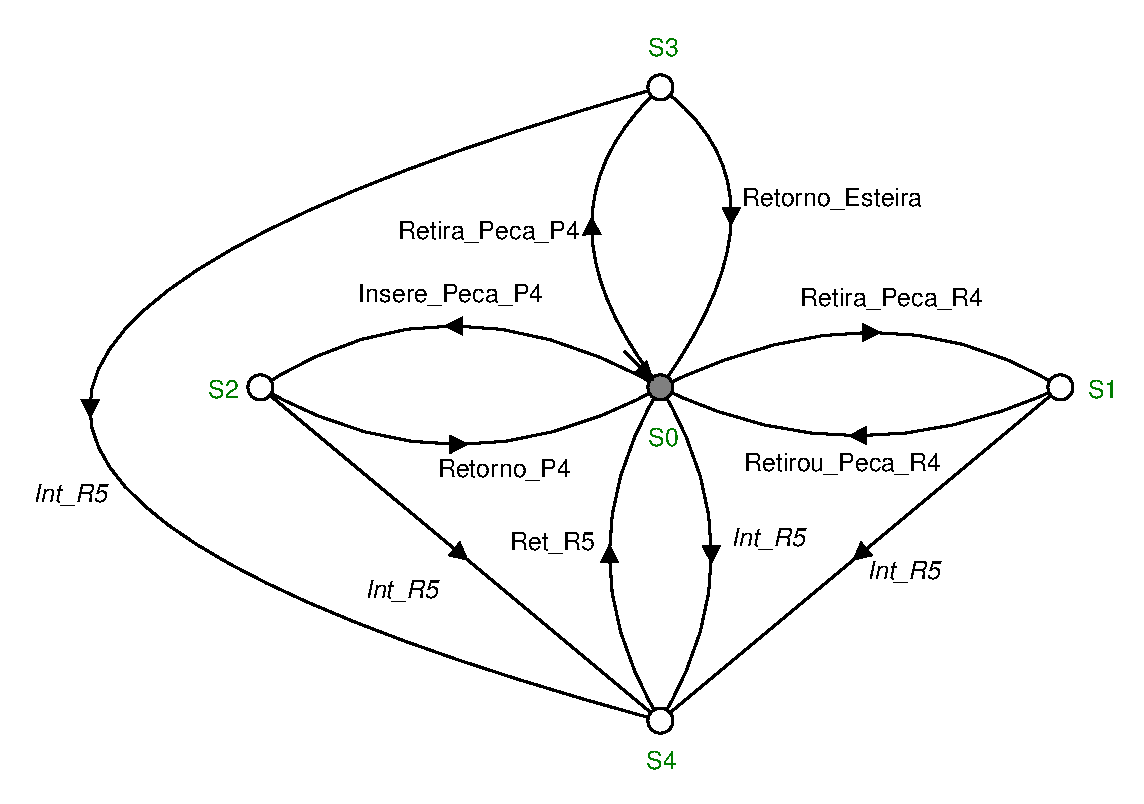
\includegraphics[width=0.9\textwidth]{imagens/robo_5.eps}
    \caption{Planta Robo 5}\label{fig:robo5}
\end{figure}

\lipsum[6]

Citação \cite{bib1} 123 456

\lipsum[7]

\section{Especificações}
\lipsum[1]
\begin{figure}[H]%
    \centering
    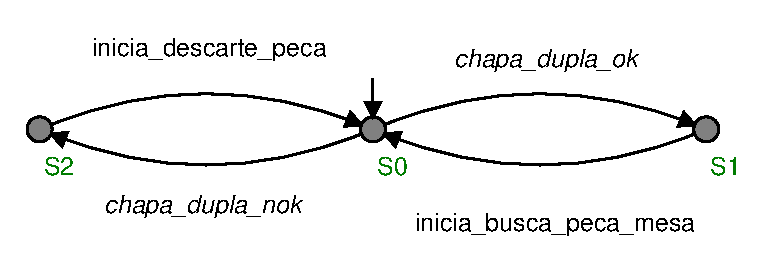
\includegraphics[width=0.9\textwidth]{imagens/E1_robo_1_chapa_dupla.eps}
    \caption{Planta Robo 5}\label{fig:robo5}
\end{figure}


\bibliography{sn-bibliography}

\end{document}
